\documentclass[12pt]{article}
\usepackage[utf8]{inputenc}
\usepackage[greek,english]{babel}
\usepackage{alphabeta}
\usepackage{fancyhdr}
\usepackage{listings}
\usepackage{mathtools}
\usepackage{xcolor}
\usepackage{float}
\usepackage{siunitx}
\usepackage[margin=0.5in]{geometry}
\usepackage[backend=bibtex]{biblatex}

\lstset {
        basicstyle=\ttfamily,
        columns=fullflexible,
        breaklines=true,
        keepspaces=true,
	showstringspaces=false
}

\title{Εργαστήριο Ασφάλειας στην Τεχνολογία της Πληροφορίας -- Εργασία 2}
\author{Χρήστος Μαργιώλης -- 19390133}
\date{Απρίλιος 2024}

\begin{document}

\begin{titlepage}
        \maketitle
        \begin{figure}[t!]
        \begin{center}
        
\includegraphics[scale=0.3]{./res/uniwalogo.png} \\
        \Large
        \textbf{Πανεπιστήμιο Δυτικής Αττικής} \\
        \large
        Τμήμα Μηχανικών Πληροφορικής και Ηλεκτρονικών Υπολογιστών
        \end{center}
        \end{figure}
\end{titlepage}

\renewcommand{\contentsname}{Περιεχόμενα}
\tableofcontents
\pagebreak

\section{Δομή αρχείων}

\subsection{Αρχεία C}

Ο κώδικας C, για δική μου διευκόλυνση στην δοκιμή διαφόρων εισόδων, περιέχει και
ρουτίνες διαβάσματος αρχείων, πέρα από την επίλυση των προβλημάτων. Τα περισσότερα
προγράμματα χρησιμοποιούνται σε συνδυασμό με κάποιο από τα scripts που αναλύονται
παρακάτω. Αυτό προσθέτει μεν πολυπλοκότητα, αλλά κάνει τα προγράμματα πιο ευέλικτα.
Σε κάθε δραστηριότητα εξηγώ πως πρέπει να τρέξουμε το πρόγραμμα.

\subsection{Scripts}

Πέρα από τον κώδικα έγραψα και τα παρακάτω 2 scripts.

\subsubsection{\lstinline{atoh}: Μετατροπή από ASCII σε Hex}

\lstinputlisting[language=c]{../src/atoh}

\subsubsection{\lstinline{htoa}: Μετατροπή από Hex σε ASCII}

\lstinputlisting[language=c]{../src/htoa}

\subsection{Makefile}

Τα προγράμματα μεταγλωττίζονται όλα αυτόματα μέσω του παρακάτω
\lstinline{Makefile}.

Το \lstinline{Makefile} διαθέτει τις παρακάτω επιλογές:
\begin{itemize}
	\item \lstinline{make}: Κάνει compile όλα τα προγράμματα.
	\item \lstinline{make clean}: Σβήνει τα εκτελέσιμα αρχεία που έχουν
		παραχθεί.
\end{itemize}

Ο κώδικας του:

\lstinputlisting[language=c]{../src/Makefile}

\subsection{Αρχεία δεδομένων}

Στο directory \lstinline{src/dat} βρίσκονται αρχεία δεδομένων που
χρησιμοποιούνται από τα προγράμματα. 'Ολα τα αρχεία ακολουθούν την ονομασία
\lstinline{<program>.in} όπου \lstinline{program} το όνομα του προγράμματος που
το χρησιμοποιεί. Προκειμένου να αποφευχθεί τυχόν περιττή πολυπλοκότητα, τα
προγράμματα δεν κάνουν ελέγχους εγκυρότητας των αρχείων εισόδου.

\section{Δραστηριότητα 1: Δημιουργία ιδιωτικού κλειδιού}

\subsection{Επεξήγηση υλοποίησης}

Για να δημιουργήσουμε ένα ιδιωτικό κλειδί RSA, πρέπει αρχικά να υπολογίσουμε
την συνάρτηση:
\[\phi(n) = (p-1)(q-1)\]
Στην συνέχεια, θα υπολογίσουμε την εξίσωση:
\[e \cdot d \mod \phi(n) = 1\]
Λύνοντας ως προς $d$. Ο υπολογισμός του ιδιωτικού κλειδιού μέσα στο πρόγραμμα
γίνεται με τις εξής εντολές: \\

\begin{lstlisting}[language=C]
	...
	BN_dec2bn(&one, "1");
	BN_sub(foo, p, one);
	BN_sub(bar, q, one);
	BN_mul(phi, foo, bar, ctx);
	BN_mod_inverse(d, e, phi, ctx);
\end{lstlisting}

\subsection{Εκτέλεση προγράμματος}

Χρήση: \lstinline{priv [-v] input} \\

Το πρόγραμμα, όταν το τρέξουμε απλώς με το αρχείο εισόδου, τυπώνει το
ιδιωτικό κλειδί. Αν του δώσουμε και την επιλογή \lstinline{-v}, τυπώνει
αναλυτικά τα $e$, $n$ και $d$. Η επιλογή αυτή είναι χρήσιμη για την
παραγωγή του αρχείου εισόδου που χρησιμοποιείται για την κρυπτογράφηση
μηνυμάτων: \\

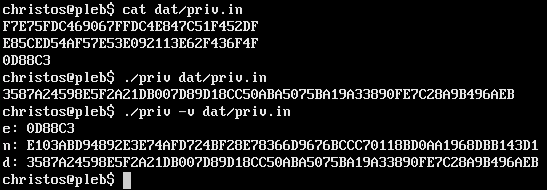
\includegraphics[width=\textwidth]{res/priv.png} \\

\subsection{Πηγαίος κώδικας: \lstinline{priv.c}}

\lstinputlisting[language=c]{../src/priv.c}

\section{Δραστηριότητα 2: Κρυπτογράφηση μηνύματος}

\subsection{Επεξήγηση υλοποίησης}

Η κρυπτογράφηση ενός μηνύματος γίνεται με τον τύπο:
\[C = P^e \mod n\]
Και η αποκρυπτογράφηση του:
\[P = C^d \mod n\]

Η συνάρτηση OpenSSL για την πράξη αυτή είναι η \lstinline{BN_mod_exp()}. Οι
παρακάτω εντολές στον κώδικα εκτελούν την (απο)κρυπτογράφηση: \\

\begin{lstlisting}[language=C]
	...
	/* Encrypt message */
	BN_mod_exp(encrstr, str, e, n, ctx);
	/* Decrypt message */
	BN_mod_exp(decrstr, encrstr, d, n, ctx);
\end{lstlisting}

\subsection{Εκτέλεση προγράμματος}

Χρήση: \lstinline{./atoh 'msg' | encrypt input} \\

Παρακάτω φαίνεται ένα ενδεικτικό τρέξιμο. Το μήνυμα μετατρέπεται σε Hex με την
χρήση του \lstinline{atoh} script. Αξίζει να σημειωθεί ότι στην υλοποίησή μου,
τα $e$, $n$ και $d$ υπολογίζονται από το \lstinline{priv.c} και
χρησιμοποιούνται κατευθείαν από το \lstinline{encrypt.c} ώστε να αποφευχθεί η
επανάληψη κώδικα, εξ'ου και η χρήση του \lstinline{priv} στην αρχή: \\

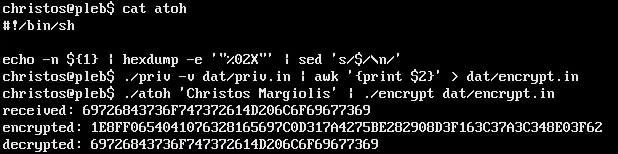
\includegraphics[width=\textwidth]{res/encrypt.png} \\

\subsection{Πηγαίος κώδικας: \lstinline{encrypt.c}}

\lstinputlisting[language=c]{../src/encrypt.c}

\section{Δραστηριότητα 3: Αποκρυπτογράφηση μηνύματος}

\subsection{Επεξήγηση υλοποίησης}

'Οπως και στην δραστηριότητα 3, χρησιμοποιείται ο ίδιος τύπος για την
αποκρυπτογράφηση ενός μηνύματος.

\subsection{Εκτέλεση προγράμματος}

Χρήση: \lstinline{decrypt input | htoa} \\

Στο αρχείο εισόδου θα χρησιμοποιήσουμε τα ίδια κλειδιά με αυτά της άσκησης 3,
συν ότι θα προσθέσουμε και το επιπλέον κρυπτογράφημα που δίνεται στην εκφώνηση
της άσκησης. Το πρόγραμμα τυπώνει το αποκρυπτογραφημένο μήνυμα σε Hex, οπότε
διοχετεύουμε την έξοδό του στο \lstinline{htoa} script ώστε να μετατραπεί σε
ASCII: \\

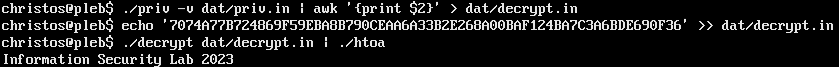
\includegraphics[width=\textwidth]{res/decrypt.png} \\

\subsection{Πηγαίος κώδικας: \lstinline{decrypt.c}}

\lstinputlisting[language=c]{../src/decrypt.c}

\section{Δραστηριότητα 4: Υπογραφή μηνύματος}

\subsection{Επεξήγηση υλοποίησης}

Η υπογραφή ενός μηνύματος γίνεται με τον τύπο:
\[S = H(P)^d \mod n\]

Στον κώδικα, η υλοποίηση γίνεται ως εξής: \\
\begin{lstlisting}[language=C]
	...
	BN_mod_exp(sign, str, d, n, ctx);
\end{lstlisting}

\subsection{Εκτέλεση προγράμματος}

Χρήση: \lstinline{atoh 'msg' | sign input} \\

Στο παρακάτω ενδεικτικό τρέξιμο, παρατηρούμε ότι μία πολύ μικρή αλλαγή στο
μήνυμα θα παράξει τελείως διαφορετική υπογραφή, οπότε είμαστε και σίγουροι ότι
τα μηνύματα δεν ήτανε ίδια: \\

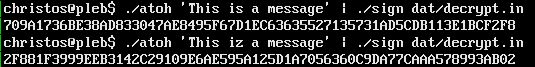
\includegraphics[width=\textwidth]{res/sign.png} \\

\subsection{Πηγαίος κώδικας: \lstinline{sign.c}}

\lstinputlisting[language=c]{../src/sign.c}

\section{Δραστηριότητα 5: Επαλήθευση υπογραφής}

\subsection{Επεξήγηση υλοποίησης}

Η επαλήθευση της υπογραφής γίνεται με τον τύπο:
\[Digest = S^e \mod n\]

Στον κώδικα, υλοποίηση είναι γίνεται ως εξής: \\
\begin{lstlisting}[language=C]
	...
	BN_mod_exp(str, sign, e, n, ctx);
\end{lstlisting}

\subsection{Εκτέλεση προγράμματος}

Χρήση: \lstinline{verify input} \\

\subsection{Περίπτωση Α}

Αρχικά θα δώσουμε ως είσοδο την έγκυρη υπογραφή: \\

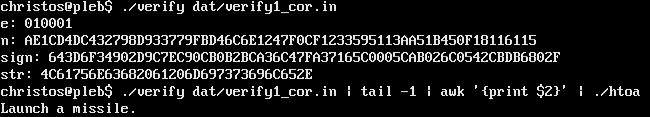
\includegraphics[width=\textwidth]{res/verify1.png} \\

'Οταν αλλάξουμε το τελευταίο byte της υπογραφής, παρατηρούμε ότι η επαλήθευση
δεν είναι έγκυρη: \\

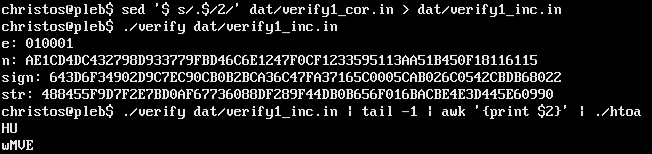
\includegraphics[width=\textwidth]{res/verify2.png} \\

\subsection{Περίπτωση Β}

Από το παρακάτω τρέξιμο, βλέπουμε ότι η υπόγραφη είναι πράγματι της Alice: \\

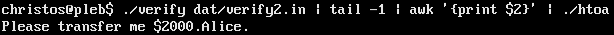
\includegraphics[width=\textwidth]{res/verify3.png} \\

\section{Δραστηριότητα 6: Μη-αυτόματη επαλήθευση πιστοποιητικού X.509}

\textit{Για την συγκεκριμένη δραστηριότητα επέλεξα να παραθέσω τις εντολές σε μορφή
text αντί για screenshots διότι τα output και οι ίδιες οι εντολές είναι πολύ
μεγάλες για να φανούν καθαρά σε εικονα.} \\

Κατεβάζουμε το πιστοποιητικό της ιστοσελίδας margiolis.net:
\begin{lstlisting}
	$ openssl s_client -connect margiolis.net:443 -showcerts \
		</dev/null 2>/dev/null | openssl x509 -outform pem > dat/c0.pem
\end{lstlisting}

Εξάγουμε το $e$:
\begin{lstlisting}
	$ openssl x509 -in dat/c0.pem -text -noout | grep 'Exponent' |
		awk '{print $3}' | sed 's/(//;s/)//;s/0x//' > dat/cert.in
\end{lstlisting}

Εξάγουμε το $n$:
\begin{lstlisting}
	$ openssl x509 -in dat/c0.pem -noout -modulus |
		sed 's/Modulus=//' >> dat/cert.in
\end{lstlisting}

Εξάγουμε την υπογραφή:
\begin{lstlisting}
	$ openssl x509 -in dat/c0.pem -text -noout \
		-certopt ca_default -certopt no_validity \
		-certopt no_serial -certopt no_subject \
		-certopt no_extensions -certopt no_signame |
		sed 1d | tr -d '[:space:]:' | sha256 >> dat/cert.in
\end{lstlisting}

Τέλος, επαληθεύουμε το πιστοποιητικό (το output είναι πολύ μεγάλο για να
συμπεριληφθεί ολόκληρο):
\begin{lstlisting}
	$ ./verify dat/cert.in
	e: 010001
	n: B8CF80904908D88..........1AE7F0DE351B
	sign: EC3CF68F5F6...........D228F04C5E54BE1D
	str: 6E7DBA8412AEB7CF.........5FE55D1059486304
\end{lstlisting}

\end{document}
